\chapter{Rollenmodell}
\label{cha:Rollenmodell}

Das Rollenmodell beschreibt die vorkommenden Rollen des Integrationsszenarios eines Fahrzeugverleihsystems (z.B. CarSharing) in ein Reiseinformationssystem.

\begin{figure*}[ht]
\centering
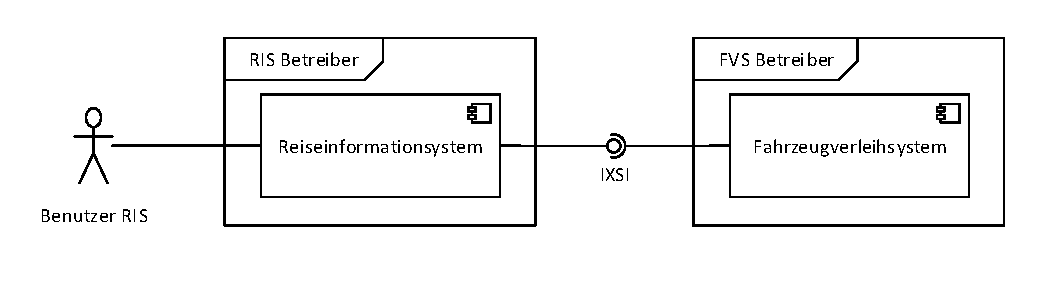
\includegraphics[width=0.8\textwidth]{ixsi.pdf}
\caption{Überblick Rollenmodell.\label{fig:Rollenmodell}}
\end{figure*}

\section{Reiseinformationssystem}
\label{sec:Rollenmodell:RIS}
\index{RIS}\index{Reiseinformationssystem}
Das Reiseinformationssystem (RIS) stellt ein Informationssystem für Reiseauskünfte dar und umfasst die Zusammenführung der Reiseangebote, die Konstruktion von Reiseketten, die Berechnung des Gesamtpreises für eine Reisekette, die Reservierung der Mobilitätsangebote für die einzelnen Elemente einer Reisekette, die Aufbereitung der Daten für die Darstellung in Benutzerschnittstellen und abschließend die Darstellung der Informationen.

\subsection*{Anwendungsfälle}
\begin{itemize}
\item Kunde fragt mit Suchbedingungen und Präferenzen Auskünfte über Mobilitätsangebote beim RIS an. Suchbedingungen und Präferenzen sind beispielsweise Start- und Zielort, Abfahrt- und Ankunftszeitpunkt, zu berücksichtigende Verkehrsmittel, Anzahl der Umstiege, Preisspanne, etc. Die Ergebnisse werden den Kunden über die Benutzerschnittstelle des RIS in Form von Reiseketten dargestellt. 
\end{itemize}

\section{Fahrzeugverleihsystem}
\label{sec:Rollenmodell:FVS}
\index{FVS}\index{Fahrzeugverleihsystem}
Das Fahrzeugverleihsystem (FVS) stellt ein Informationssystem zur Verwaltung und Buchung von Leihfahrzeugen und Kunden dar. Fahrzeuge können sowohl unterschiedlichen Typs, als auch Stationsgebunden oder -ungebunden sein.

\subsection*{Anwendungsfälle}
\begin{itemize}
\item Ein Kunde bucht (leiht) über das FVS ein Fahrzeug zu vertraglich geregelten Preisen, Zeiten und Stationen aus und nutzt dieses.
\item Ein Kunde fragt über das FVS die Vefügbarkeit eines Fahrzeugs an. 
\end{itemize}

\section{Benutzer RIS}
\index{Benutzer!RIS}
Kunde RIS – stellt eine juristische Person dar, die befugt ist eine Reise zu buchen und unter Nutzung der gewählten Verkehrsmittel, anzutreten. 

\subsection*{Anwendungsfälle}
\begin{itemize}
\item Benutzer stellt Auskunftsanfrage an das RIS.
\item Benutzer bucht Reise über das RIS.
\end{itemize}

\section{Benutzer FVS}
\index{Benutzer!FVS}
Kunde FVS - stellt eine juristische Person dar, die befugt ist ein Fahrzeug zu leihen und zu nutzen.

\subsection*{Anwendungsfälle}
\begin{itemize}
\item Benutzer stellt Auskunftsanfrage an das FVS.
% \item Benutzer reserviert ein Fahrzeug über das FVS.
\item Benutzer bucht ein Fahrzeug über das FVS.
\end{itemize}

\section{Betreiber RIS}
\index{Betreiber!RIS}
Betreiber RIS – stellt das RIS als Informationssystem für einen Mobilitätsanbieter als Dienstleistung bereit.

% \subsection{Anwendungsfälle}

\section{Betreiber FVS}
\index{Betreiber!FVS}
Betreiber FVS - stellt ein Informationssystem für FVS für einen Fahrzeugverleiher als Dienstleistung bereit.

% \subsection{Anwendungsfälle}

% \section{FVS-Standort}
% 
% Ein FVS-Standort (z.B. eine CarSharing-Station) stellt die Fahrzeuge eines Mobilitätsanbieters an einem Ort bereit.
% 
% % \subsection{Anwendungsfälle}
% 
% \section{Fahrzeug}
% 
% Fahrzeug – wird vom Mobilitätsanbieter über das FVS an einer Station als Mobilitätsangebot für den Kunden angeboten.

% \subsection{Anwendungsfälle}
